\appendix
\label{app:class}
\chapter{CLASSIFICATION AND FEATURE EXTRACTION TECHNIQUES USED}
\section{Classification Techniques}
\subsection{Gaussian Mixture Model}
In statistics, a mixture model is a probabilistic model for representing the presence of subpopulations within an overall population. As the name indicates, train data is modeled as a mixture of Gaussian functions. This is basically linear superposition of Gaussians in the form\\
 \begin{equation}
 p(x) = \sum_{k=1}^{K}\pi_{k}N(x|\mu_{k},\Sigma_{k})
 \end{equation}
The biggest advantage of clustering using Gaussian mixture model over traditional clustering method is that each point can be represented more than one cluster. So, it is kind of best way to represent multi modality in a system. Three parameters in Gaussian mixture model, namely $\Sigma$ (covariance), $\mu$ (mean) and $\pi$ (component proportion) are estimated using expectation maximization (EM) method. EM algorithm has applications in a wide variety of tasks and has been used in the context of various machine learning models. The assumption that Gaussian mixture models take is that all the points are identically and independently distributed. So, the log of likelihood of Eqn (1) over all the points is given by
\begin{equation}
ln p(X|\pi, \mu, \Sigma) = \sum_{n=1}^{N}ln \sum_{k=1}^{K}\pi_{k}N(x|\mu_{k},\Sigma_{k})
\end{equation}  
Now the parameters of the model are estimated by maximizing this log likelihood function over an iterative procedure. This is kind of chicken and egg problem where we first input a set of parameters to the model and in return we get an improved set of parameters. This is done until the point of convergence. The initial set of parameters given to the problem are not selected randomly but are generally the output of k-means clustering. A sample mixture of Gaussians can be viewed in figure \ref{fig:gmm}.
\begin{figure}[!htbp]
\centering
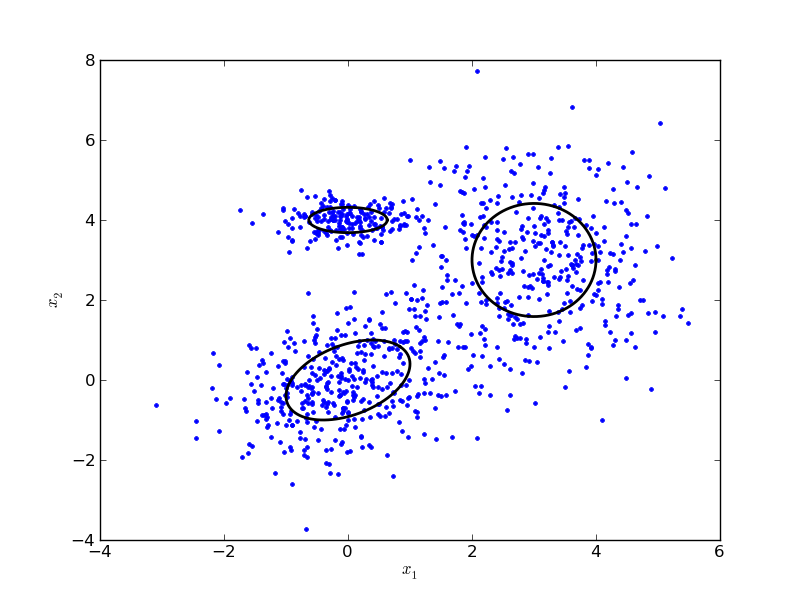
\includegraphics[scale=0.4]{snaps/sample_gmm.png}
\caption{A sample mixture of Gaussians}
\label{fig:gmm}
\end{figure}
\subsection{Hidden Markov Model (HMM)}
Most of the classifiers used in machine learning do not consider the sequence information present in data and they just consider the data as static. The problems that have inherent temporality in them and consists of process that unfolds in time, HMMs have found great use in such problems.\par
The model in HMM is represented by a three-member tuple involving the initial state probabilities, state transition probabilities and observation symbol probabilities. Initial state probabilities define the probability of starting from a particular state. State transition probabilities define the probability of transition from one state to another. Observation probabilities define the probability of observing a symbol from every state.\par
Three major issues of hidden Markov model are:
\begin{itemize}
\item Testing
\item Finding optimal state sequence
\item Training
\end{itemize}
The good news here is that all the three problems are solved and if we have set of observation sequence, then we can define all the three tuples of Hidden Markov Model. We used HTK toolkit for training HMM devised by \cite{HTK}. \par
Two kinds of HMMs used today are Discrete HMMs and continuous density HMMs. In discrete HMMs, observation probabilities in each state are discrete but on the other hand, in continuous density HMM, observation probability is a Gaussian or mixture of Gaussian with its usual parameters.  
\subsection{Support Vector Machine (SVM)}
Support vector machine is one of the most important classifiers in machine learning today. The discussion on support vector machine started after the arrival of perceptron algorithm which focused on obtaining a separating hyperplane between two classes which are linearly separable. But the difference is, Support Vector Machine instead of obtaining just a hyperplane tries to obtain a maximal margin hyperplane. This means that the hyperplane is situated exactly between corner points (also called support vectors) of the two classes. Hyperplane that we need in support vector machine is such that distance of obtained hyperplane from the support vectors of both the classes is maximum from both the classes.  \par
But in a real world, there is hardly any data where the two classes are linearly separable. So, if the data of two classes is overlapping, there is a provision of error in support vector machines. The amount of error tolerance can be specified while training the model. Although in a real world, Support Vector Machines are hardly used in actual data space. This is because of the fact that real world data is not linearly separable. Also as per Cover's theorem, \textit{A pattern recognition problem when cast in higher dimensional space is more likely to be linearly separable than in lower dimensional space.} So, the data is first moved into kernel space which is higher dimensional space or even can be infinite dimensional space. Now in this space, a maximal separating hyperplane is found. Results obtained from support vector machine is highly dependent on parameters given to it. Two of the parameters given to it are kernel width and error tolerance.

\subsection{Random Forest and Decision Trees}
The decision tree is amongst one of the important classifiers in machine learning today. Based on the training data, this algorithm creates a tree where every node from root to leaf gives a decision of which class should the test data belong to. Choice of decision at every node is based on the statistical parameters like variance in the training data. Usually, training time for decision tree is huge, so it is not used when the dataset is large. If we somehow can reduce the size of dataset, then it can be used. \par 
The decision tree is generally not used alone but is used in combination of many. Such a combination of decision trees is known as random forest. Decision given by most number of decision trees is considered to be the final decision.
\section{Feature Extraction}
\subsection{Mel Frequency Cepstral Coefficients (MFCC)}
In sound processing, the mel-frequency cepstrum is a representation of the short-term power spectrum of a sound, based on a linear cosine transform of a log power spectrum on a nonlinear mel scale of frequency.\par
Mel-frequency cepstral coefficients (MFCCs) are coefficients that collectively make up Mel Frequency Cepstrum (MFC). They are derived from a type of cepstral representation of the audio clip which is a nonlinear "spectrum of spectrum". The difference between the cepstrum and the MFC is that in the latter, the frequency bands are equally spaced on the mel scale, which approximates the human auditory system's response more closely than the linearly-spaced frequency bands used in the normal cepstrum. This frequency warping allows for better representation of sound, like in audio compression. MFCCs are commonly derived as follows:
\begin{enumerate} 
\item Take the Fourier transform of (a windowed excerpt of) a signal.
\item Map the powers of the spectrum obtained above onto the mel scale, using triangular overlapping windows.
\item Take the logs of the powers at each of the mel frequencies.
\item Take the discrete cosine transform of the list of mel log powers, as if it were a signal.
\item The MFCCs are the amplitudes of the resulting spectrum.
\end{enumerate}

\subsection{Melody (Pitch)}
Melody extraction is the task of automatically estimating the fundamental frequency corresponding to the pitch of the predominant melodic line of a piece of polyphonic music. Melody extraction is a process of estimating when melody is present and when it is not. It is also a process of estimating correct pitch when the melody is present. The current pitch extraction algorithm used in the work is devised by \cite{justin}.


